\documentclass[pdftex,12pt,a4paper]{article}
\usepackage[pdftex]{graphicx}
\usepackage{fancyhdr}
\usepackage{geometry}
\usepackage{draftcopy}
\usepackage{float}
\usepackage{amsmath}
\usepackage{algorithm2e}
\usepackage{color, colortbl}
\definecolor{Gray}{gray}{0.9}
\renewcommand{\thesection}{\arabic{section}.}
\renewcommand{\thesubsection}{\arabic{section}.\arabic{subsection} }
\renewcommand{\headrulewidth}{0pt}
\renewcommand{\footrulewidth}{0.5pt}
\pagestyle{fancy}
\fancyhead{}
\fancyfoot[LE,LO]{\footnotesize{
SE344, Chemistry and Our Environment
}
}

\title{\vspace{-15pt}Fate of Chemicals\\ SE344: Chemistry and Our Environment}
\author{Ankesh Kumar Singh (Y9090)}
\date{9th March, 2013}
\begin{document}
\maketitle
\begin{tabular}{p{370pt}}
\textbf{Keywords: }weak acid buffer, metal ion toxicity, clay adsorption, diclofenac, extinction of vultures
\end{tabular}
\vspace{10pt}\\
\hrule
\vspace{10pt}
Predicting fate of chemicals in environment is important as any new process is centered around a new material. Making accurate predictions is a very difficult task and requires a wholistic picture of the chemistry involved in the environment. Every prediction requires some model. One such model is octanol water partition coefficient. It is the ratio of equilibrium concentration of a chemical in octanol to that in water. It is an important parameter to determine whether a given chemical will be absorbed by the living systems, since the cell membrane is hydrophobic.

However, octanol water partition coefficient assumes that the molecule was completely unaffected by any interaction with the surroundings. This is usually not the case.

Another example is that of weak acids. Presence of weak acids (obtainable from a number of wastes) and strong bases (usually from soaps and detergents) leads to formation of a buffer solution. A buffer solution resists changes in pH. Thus if such a solution is left into the drains, some bacteria will not be able to survive, where as those favored by that pH will multiply in large numbers.

Chemicals left in the environment do not always remain in their free state. Evolving bacterial systems have been able to metabolize many man made chemicals like insecticides. Chemicals undergo ionic or covalent interactions that lead to the formation of different chemical species. This phenomenon is called speciation. Many organic compounds combine with metal ions to form coordination complexes. Metal ions like copper and mercury are toxic. However, ions of their coordination complex are non toxic. Thus formation of complexes with compounds like chelating agents leads to reduction of toxicity.

Adsorption property of clay leads to a similar effect. Clay has high ability to adsorb materials due to presence of silica. Parakeets of amazon eat seeds of various plants that are highly poisonous and then pick up a certain amount of clay. The clay could complex the toxins present in the seed and the carbohydrates are readily dissolved by the body. Adsorbed products exhibit differential rates of hydrolysis.

Another important case study to the fact that prediction of effect of a certain chemical on ecosystem is difficult, is the role of diclofenac in alarming depletion of vulture population. Diclofenac is a widely used pain killer for humans. It was also used in abundance in animal husbandry. The compound was sustained in the body of animals, and when their meat was consumed by vultures. It resulted in their death. 90\% of the vultures killed were nesting birds, and hence their offsprings also died of starvation. Griffon vultures that were present in a number of tens of million in India are likely to be extinct in a decade.
\begin{center}
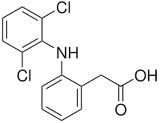
\includegraphics[scale=0.6]{diclo.jpg}
\end{center}

An important lesson is to be learnt from this story. It does not suffice to say that if a chemical is toxic to humans or plants it should not be used. If it is toxic to anyone, it is potentially dangerous. Thorough risk assessment is required before such a chemical is put to any kind of use.
\end{document}